\chapter{Materiais e Métodos}
\label{cap:metodologia}

% figuras estão no subdiretório "figuras/" dentro deste capítulo
\graphicspath{\currfiledir/figuras/}

%=====================================================

Este capítulo descreve o método utilizado no desenvolvimento do projeto, a arquitetura  e a tecnologia preconizada para a solução e, em ênfase, o processo de definição do cálculo de similaridade entre os usuários a partir do peso da aresta de um grafo.

\section{Método de desenvolvimento}

O produto foi desenvolvido pelo modelo gestão de projetos por cascata. A priorização das atividades foi baseada na competência da equipe em cada área de desenvolvimento. Dessa maneira, o \emph{front end} foi considerado o foco e a prioridade no desenvolvimento, tendo em vista que o nível de conhecimento da equipe na área de design e usabilidade era perceptivelmente menor do que a habilidade para o desenvolvimento do \emph{back end}.

Na Figura \ref{fig:cascata}, estão as fases implementadas do modelo em cascata as quais foram aplicadas no desenvolvimento do sistema. Note-se iteração das fases de desenvolvimento e verificação, que representa a recorrência da atividade de implementar uma funcionalidade e imediatamente testá-la. Apesar de haver iteração não foi empregado método ágil de desenvolvimento uma vez que não se observou entrega de valor parcial.

\begin{figure}[!htb]
\centering
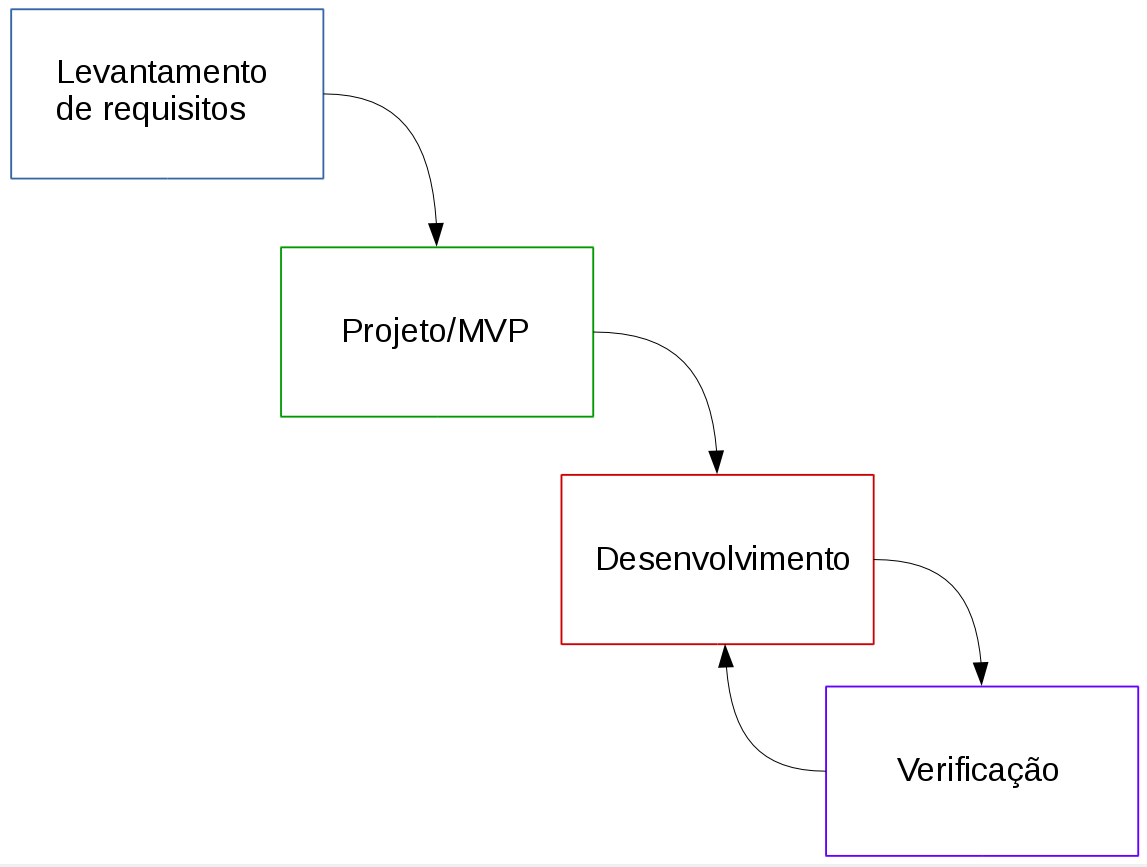
\includegraphics[width=10cm]{cascata.png}
\caption{Fases empregadas do modelo em cascata. Fonte: os autores.}
\label{fig:cascata}
\end{figure}

\subsection{Análise de requisitos}

Um MVP, sigla para \emph{Minimum Viable Product}, ou seja, um produto mínimo viável foi desenvolvido durante a fase de levantamento de requisitos. O MVP é um software com a menor quantidade possível de funcionalidades que ainda poderia entregar valor ao usuário. A Figura \ref{fig:mvpCriarQuest} apresenta a tela de criação de perguntas do MVP. Neste produto, é possível criar perguntas (\ref{fig:mvpCriarQuest}), responder perguntas postadas por outros usuários (\ref{fig:mvpVerQuest}) e marcar essas respostas (\ref{fig:mvpVerResp}). Assim, o produto já tem informações suficientes para criar um grafo com os usuários no qual o peso das arestas é o nível de afinidade entre os eles baseado na quantidade de respostas marcadas.

\begin{figure}[!htb]
\centering
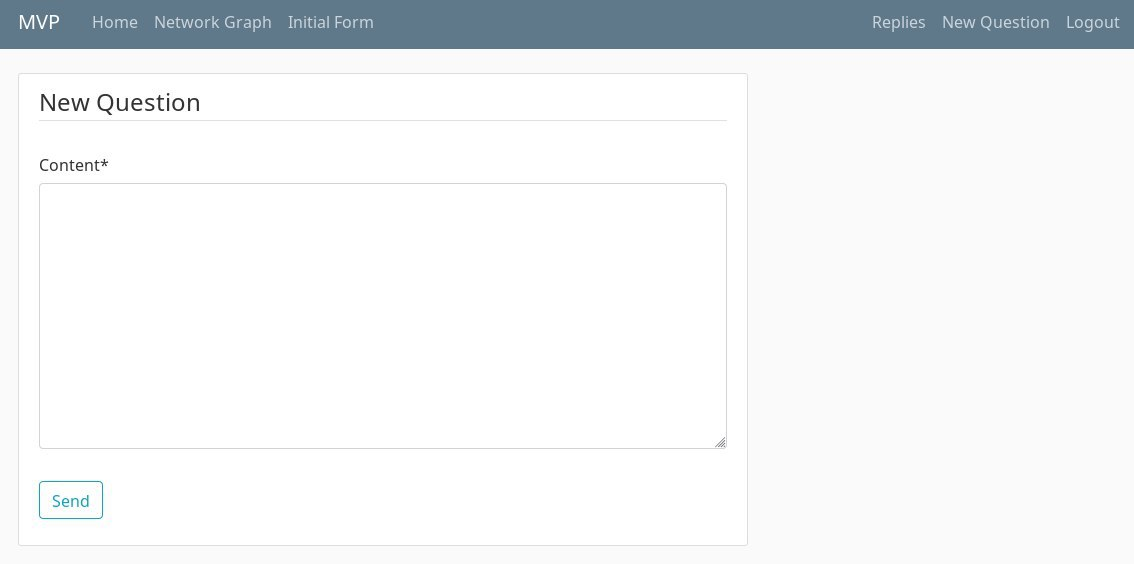
\includegraphics[width=14cm]{mvpCriarQuest.png}
\caption{Tela de criação de perguntas do MVP. Fonte: os autores.}
\label{fig:mvpCriarQuest}
\end{figure}

\begin{figure}[!htb]
\centering
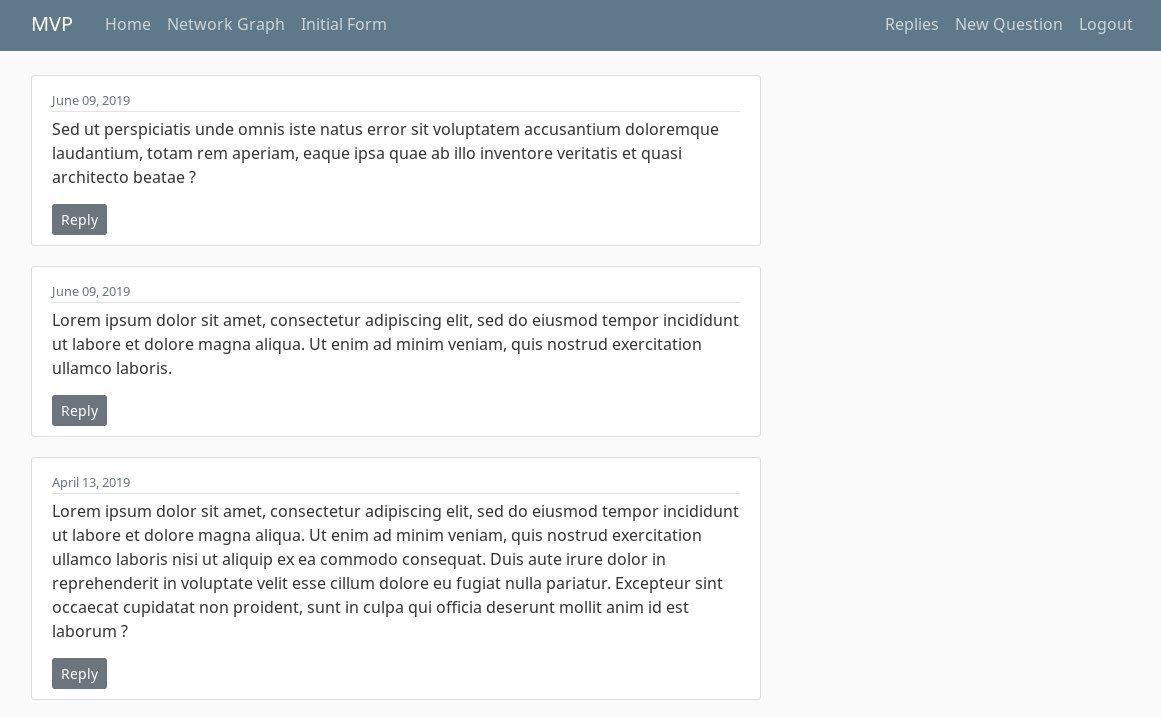
\includegraphics[width=14cm]{mvpVerQuest.png}
\caption{Tela de visualização de perguntas do MVP. Nesta tela é possível escolher uma pergunta para ser respondida. Fonte: os autores.}
\label{fig:mvpVerQuest}
\end{figure}

\begin{figure}[!htb]
\centering
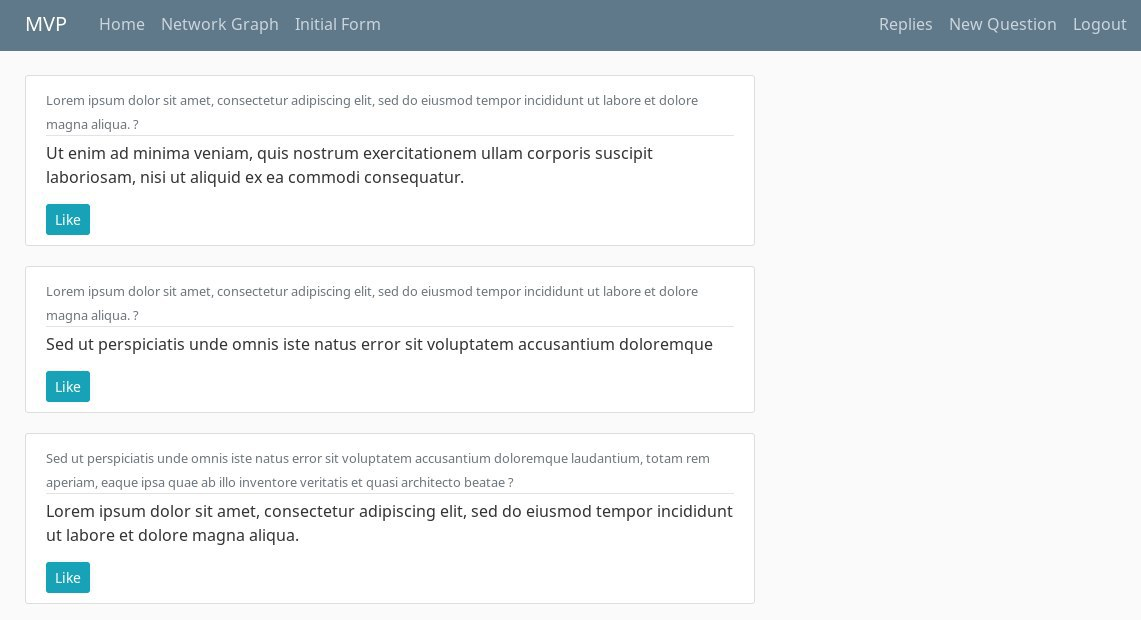
\includegraphics[width=14cm]{mvpVerResp.png}
\caption{Tela de visualização de respostas recebidas do MVP. Nesta tela é possível marcar perguntas favoritas. Fonte: os autores.}
\label{fig:mvpVerResp}
\end{figure}

\begin{figure}[!htb]
\centering
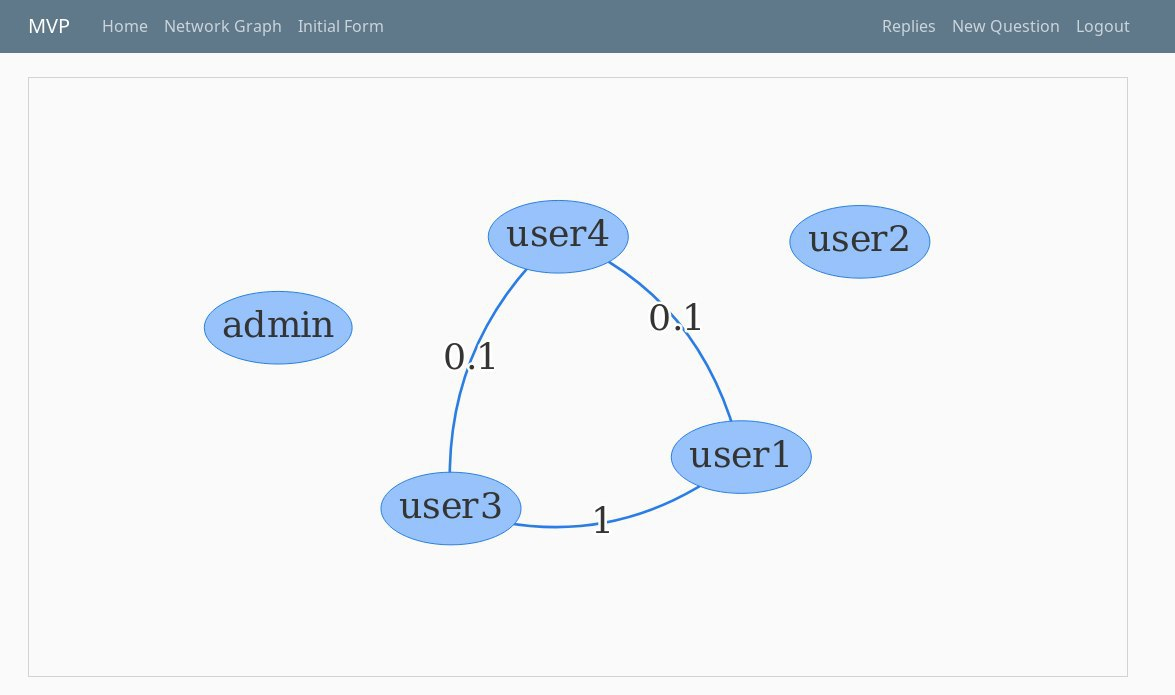
\includegraphics[width=14cm]{mvpVerGrafo.png}
\caption{Visualização do grafo que representa as ligações entre usuários da rede social no MVP. Fonte: os autores.}
\label{fig:mvpVerGrafo}
\end{figure}

As Figuras \ref{fig:mvpCriarQuest}, \ref{fig:mvpVerQuest} e \ref{fig:mvpVerResp} são as telas implementadas com as funções de criar questão, ver questão e ver respostas, respectivamente. Neste MVP os usuários são representados por um grafo no qual cada usuário é um nó e o peso das arestas que ligam dois nós é o valor que representa o grau de afinidade entre dois usuários. Definindo o peso da aresta como sendo $k$, o seu valor foi calculado com a seguinte equação: 

\begin{equation}
k_{ab} = \frac{R_{ab}+R_{ba}}{P_{a} + P_{b}}
 \label{eq:k-1}
\end{equation}

Onde $R_{ab}$ e $R_{ba}$ são o número de respostas dadas pelo usuário $A$ e pelo usuário $B$, respectivamente; e $P_{a}$ e $P_{b}$ são o número de perguntas criadas pelo usuário $A$ e $B$, respectivamente.

O cálculo de $k$ é tratado com atenção na Seção 3.5, onde passamos por várias funções e discutimos os pontos fortes e fracos de cada possibiliade.

A Figura \ref{fig:mvpVerGrafo} é a tela do MVP que representa os usuários e suas conexões criadas na rede social por meio de um grafo. Esta tela mostra todos os usuários cadastrados na rede social como os nós do grafo e as respectivas conexões como as arestas. O valor mostrado nas arestas é nível de afinidade entre os usuários.
\FloatBarrier

Depois do MVP, as telas principais foram prototipadas com o uso do software Pencil. Todas as telas que seriam implementadas foram desenhadas na fase de levantamento de requisitos. Neste momento, foi decidido que a aplicação teria 5 telas principais, sejam elas:

\begin{itemize}
\item Visualizar perguntas. (Figura \ref{fig:prot_perguntas})
\item Escrever perguntas. (Figura \ref{fig:prot_escreverPergunta})
\item Escrever respostas. (Figura \ref{fig:prot_escreverResposta})
\item Visualizar respostas. (Figura \ref{fig:prot_respostas})
\item Visualizar contatos. (Figura \ref{fig:prot_conversas})
\end{itemize}


\begin{figure}
\centering
\begin{minipage}{0.45\textwidth}
\centering
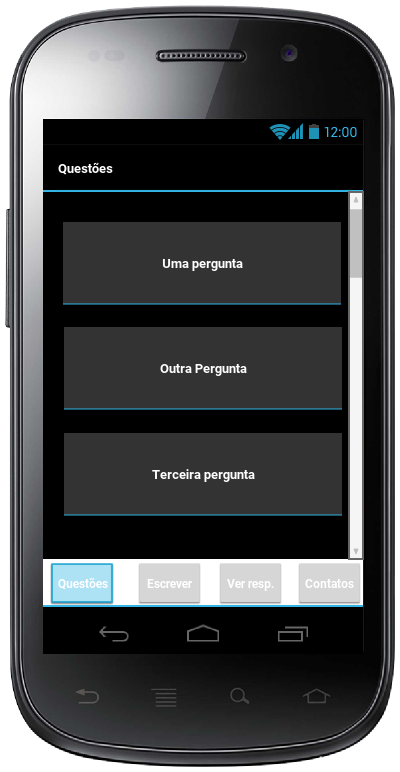
\includegraphics[width=5cm]{protperguntas.png}
\caption{Protótipo da tela de visualização de perguntas. Fonte: os autores.}
\label{fig:prot_perguntas}
\end{minipage}\hfill
\begin{minipage}{0.45\textwidth}
\centering
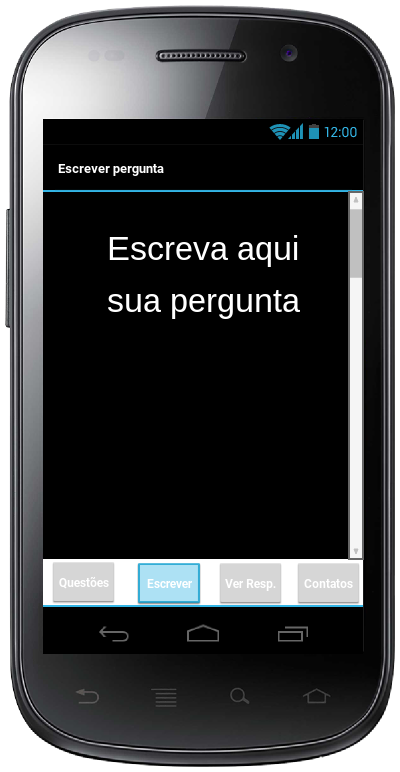
\includegraphics[width=5cm]{protescreverpergunta.png}
\caption{Protótipo da tela de criação de perguntas. Fonte: os autores.}
\label{fig:prot_escreverPergunta}
\end{minipage}
\end{figure}


\begin{figure}
\centering
\begin{minipage}{0.45\textwidth}
\centering
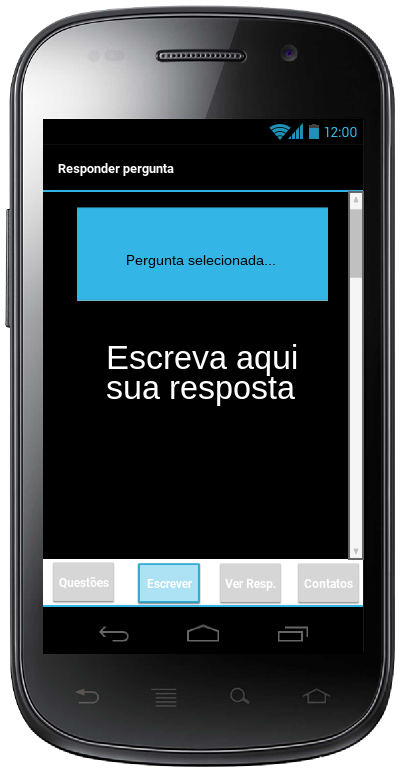
\includegraphics[width=5cm]{protescreverresposta.png}
\caption{Protótipo da tela de criação de respostas para as perguntas apresentadas. Fonte: os autores.}
\label{fig:prot_escreverResposta}
\end{minipage}\hfill
\begin{minipage}{0.45\textwidth}
\centering
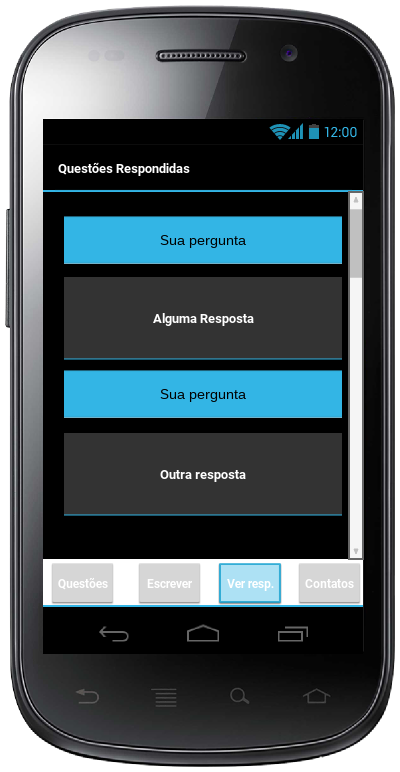
\includegraphics[width=5cm]{protrespostas.png}
\caption{Protótipo da tela de visualização das respostas dadas às perguntas produzidas pelo usuário. Fonte: os autores.}
\label{fig:prot_respostas}
\end{minipage}
\end{figure}

\begin{figure}
\centering
\begin{minipage}{0.45\textwidth}
\centering
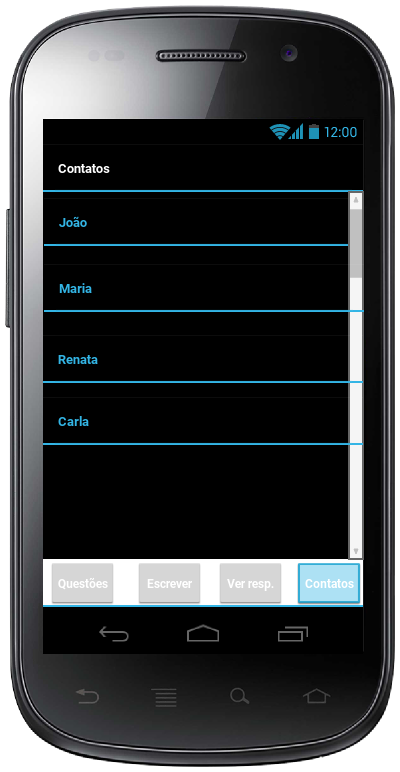
\includegraphics[width=5cm]{protconversas.png}
\caption{Protótipo da tela de visualização dos contatos. Fonte: os autores.}
\label{fig:prot_conversas}
\end{minipage}\hfill
\begin{minipage}{0.45\textwidth}
\centering
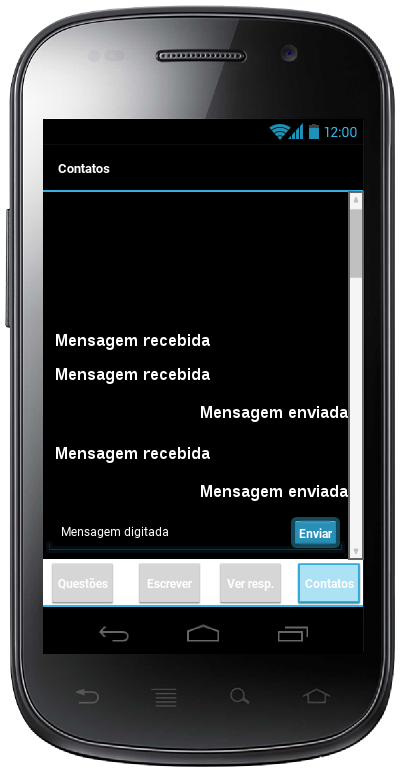
\includegraphics[width=5cm]{prot_chat.png}
\caption{Protótipo da tela de mensagens instantâneas. Fonte: os autores.}
\label{fig:prot_chat}
\end{minipage}
\end{figure}

\FloatBarrier

Foi definida, a partir da análise dos requisitos, a seguinte ordem de desenvolvimento:

\begin{enumerate}
\item Desenhar telas
\begin{enumerate}
\item Login
\item Registro
\item Criação de perguntas
\item Visualização de perguntas
\item Criação de respostas
\item Visualização de respostas
\end{enumerate}
\item Desenvolvimento do \emph{back end}
\begin{enumerate}
\item Criação do banco de dados
\item Criação de perguntas
\item Visualização de perguntas
\item Criação de respostas
\item Visualização de respostas
\end{enumerate}
\end{enumerate}



\section{Arquitetura}

% \begin{itemize}
% \item Qual a tecnologia
% \item Custo
% \item Arquitetura
% \end{itemize}

O software foi concebido para ter capacidade multi-plataforma. Desta maneira, ele pode ser acessado via \emph{browser}, aplicação Android ou IOS. A aplicação, ou página web, faz requisições para o servidor via protocolo http.

Na Figura \ref{fig:arquitetura}, há a arquitetura geral da aplicação e o diagrama de implementação na mesma ilustração.

\begin{figure}[!htb]
\centering

\includegraphics[width=14cm]{arquitetura.png}
\caption{Diagrama de implementação. Fonte: os autores.}
\label{fig:arquitetura}
\end{figure}

Neste conceito, o cliente faz uma requisição ao servidor e fornece o seu \emph{token} de identificação. Os dados inseridos pelo usuário são, a partir da interface, transportados pelas classes do pacote Models para o pacote Page respectivo, dependendo do tipo de requisição. O pacote Pages chama uma classe do pacote Services que fará a requisição ao servidor no modelo que é compreendido pela API Controller. Este pacote usa Models do lado do servidor para requisitar do banco de dados as informações solicitadas inicialmente pelo cliente. Os dados são transformados pelo pacote Serializer que os transforma em um objeto JSON que é enviado novamente ao cliente.
%=====================================================

\section{Tecnologia aplicada}

% \begin{itemize}
% \item Linguagens de programação
% \item Frameworks
% 
% \end{itemize}

O software foi implementado usando o \emph{framework} Ionic \citep{ionic}, para o \emph{front end} e o Django \citep{django}, para a camada de acesso aos dados. Essa decisão facilitou o desenvolvimento da interface, uma vez que o Ionic tem boas funcionalidades para esse fim, e possibilitou uma rápida integração com o servidor a partir do Django.

Do lado cliente, o \emph{framework} Ionic utiliza as linguagens Typescript, JavaScript, HTML, CSS e o Angular Template Syntax. No servidor a linguagem utilizada é Python e o sistema gerenciador de banco de dados é o PostgreSQL.

O Ionic é um \emph{framework} de desenvolvimento multi-plataforma, o que possibilita o desenvolvimento de aplicações que podem ser utilizadas em equipamentos com sistema operacional Android, IOS ou os navegadores Chrome, Safari, Edge, Firefox e Internet Explorer 11 ou superior. A escolha por este \emph{framework} para o desenvolvimento do software neste trabalho é baseada, essencialmente, na facilidade de criar uma aplicação multi-plataforma e no fato de ser uma ferramenta \emph{opensource}. Tendo em vista que nenhum dos desenvolvedores do grupo tinha experiência em desenvolvimento \emph{mobile}, a decisão pelo Ionic mostrou-se acertada pois a curva de aprendizado é evidentemente acentuada no início da utilização. Outra vantagem clara comparativamente ao desenvolvimento Android nativo, é que o \emph{framework} requer consideravelmente menos recurso do que um SDK como o Android Studio, por exemplo.

O Django foi utilizado neste trabalho para o desenvolvimento da camada de acesso aos dados. É completamente desenvolvido na linguagem de programação \emph{Python} sob o padrão de arquitetura \emph{Model-View-Controller}. A preferência pelo Django também está relacionada ao fato deste ter código aberto. Além disso, os integrantes da equipe já tinham experiência no uso do Django e essa facilidade era uma conveniência que não podia ser desprezada.

O versionamento e o compartilhamento do desenvolvimento foi realizado como uso do GitHub.

O desenvolvimento foi realizado em uma estação de trabalho do modelo PC Notebook Thinkpad X201, cujas especificações são as seguintes.

\begin{itemize}
\item Disco: SSD 120GB.
\item Memória RAM: 8GB
\item Processador: Intel I5-540M (2.53GHz, 3MB Cache)
\item Sistema Operacional: Arch Linux
\end{itemize}
 
O servidor foi dimensionado e deve ser administrado por um serviço de VPS, ou \emph{Virtual Private Server}, que é um serviço de hospedagem para pequenas aplicações pago. A seguir, estão as especificações preconizadas para o software:

\begin{itemize}
\item Memória RAM: 2GB
\item Processador: Intel Haswell 2.3GHz
\item Sistema Operacional: Debian Stretch
\end{itemize}

O container que sustenta a aplicação dentro do servidor, será administrado com o uso da ferramenta Docker.
%=====================================================

\section{Análise do sistema}

O primeiro passo da análise do sistema foi a definição dos casos de uso. No Apêndice A estão os diagramas de caso de uso, os diagramas de sequência e as especificações dos casos de uso.

As classes definidas estão ilustradas na Figura \ref{fig:diagramaClasse}. A estrutura de dados que representa o usuário tem as relações com os seus vizinhos no grafo representadas por um \emph{link} que carrega o nome do vizinho e o valor de $k$. Dessa maneira, temos classes definidas de modo que $User$ está relacionado a $Neighbor$ por uma lista de adjacência, uma vez que existe uma relação de muitos para muitos.

\begin{figure}[!htb]
\centering
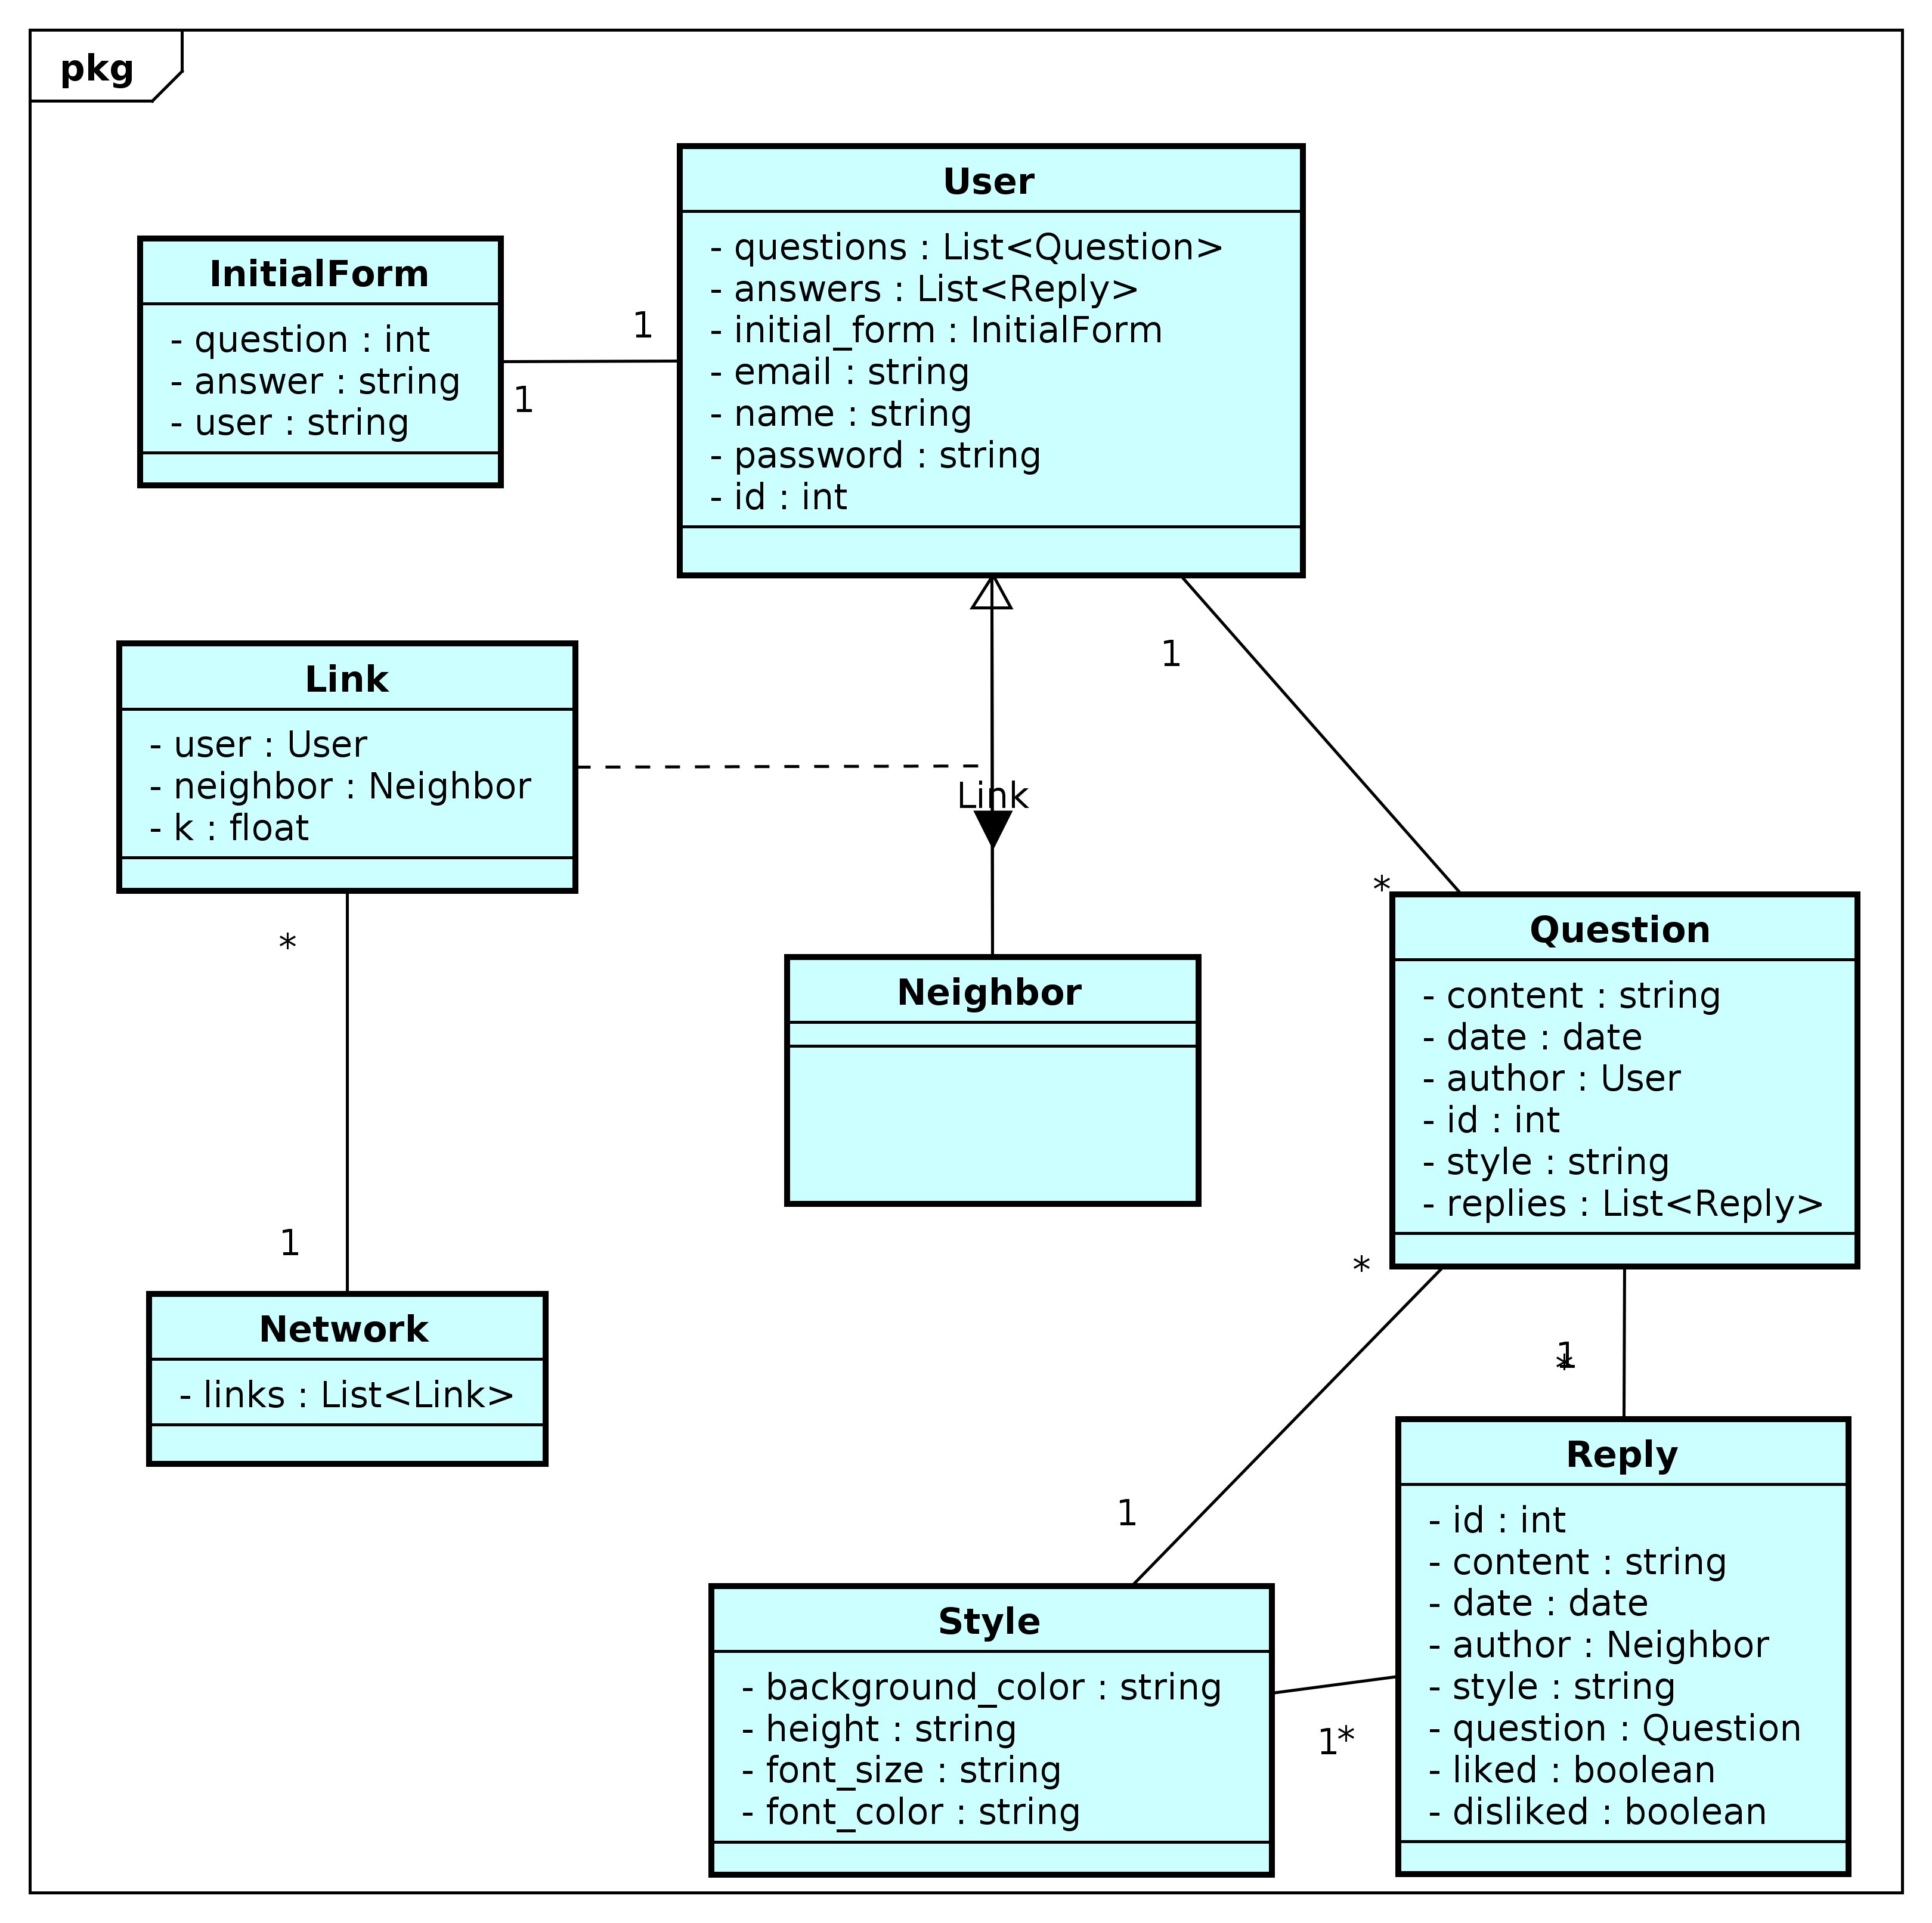
\includegraphics[width=16cm]{DiagramaClasse.png}
\caption{Diagrama de classes. Fonte: os autores.}
\label{fig:diagramaClasse}
\end{figure}

A Figura \ref{fig:diagramaBD} é o diagrama do Banco de Dados. Sabendo que o \emph{framework} Django foi utilizado para desenvolver as conexões com o banco de dados e este utiliza o arquitetura \emph{Model-View-Controller}, as entidades são muito semelhantes às classes, pois as classes definem os objetos do \emph{model}.

\begin{figure}[!htb]
\centering
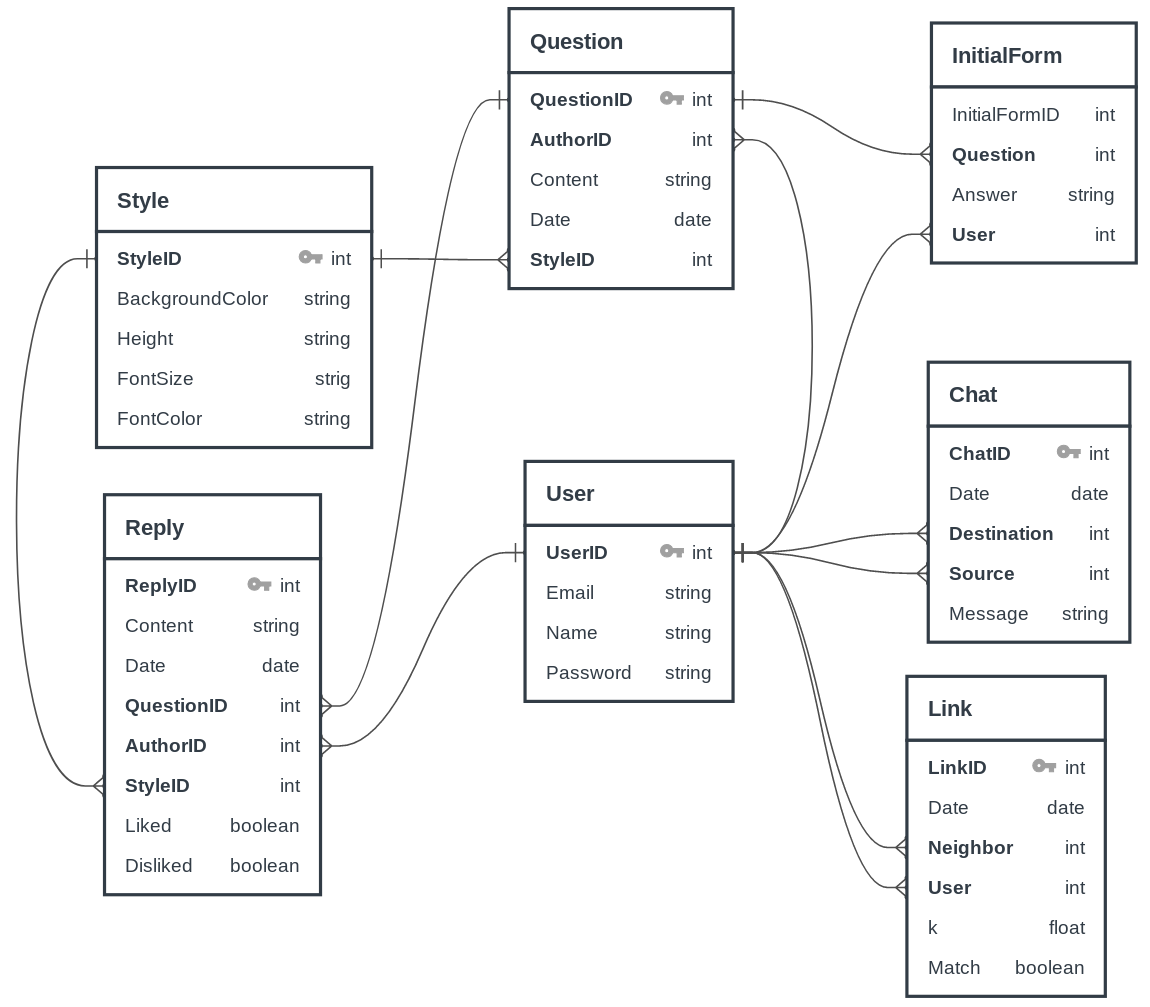
\includegraphics[width=16cm]{diagrama_bd.png}
\caption{Diagrama de banco de dados. Fonte: os autores.}
\label{fig:diagramaBD}
\end{figure}

\FloatBarrier


%=====================================================

\section{Cálculo do peso da aresta}
O peso de uma aresta do grafo, $k$, representa o nível de afinidade entre os dois usuários conectados por esta aresta. Um usuário pode estar conectado a vários outros usuários.

Quando um usuário entra pela primeira vez na rede social, ele é obrigado a preencher um questionário contendo as questões constantes na Tabela \ref{tab:questoes}. A partir das respostas deste questionário, um valor para $k$ é calculado levando em conta, tão somente, a similaridade entre as respostas de cada usuário.

\begin{table}[!htp]
\centering
\caption{Formulário inicial}
\label{tab:questoes}
\begin{tabular}{ | c |}
\hline
Pergunta\\
\hline
\hline
Você prefere cachorro ou gato?\\  
\hline
Você prefere rock ou funk?\\
\hline
Você prefere verão ou inverno? \\
\hline
Você prefere cinema ou teatro?\\
\hline
Você prefere cerveja ou vinho?\\
\hline
Você prefere o dia ou a noite?\\
\hline
Você prefere sair ou ficar em casa?\\
\hline
Você fuma?\\
\hline
Você tem alguma religião?\\
\hline
Você acredita em signos?\\
\hline
Você prefere praia ou campo?\\
\hline
\end{tabular}
\end{table}

As perguntas elaboradas para o formulário em \ref{tab:questoes}, são simplificadas para não exaurir o usuário em sua primeira utilização do software. Essas perguntas podem ser melhor elaboradas a partir dos resultados obtidos ao longo da vida do software ou podem ser regionalizadas para atender melhor cada nicho de usuários. Como o objetivo deste trabalho não é fazer a análise sociológica dos interesses dos usuários, não foi despendido esforço maior para otimizar essas questões.

Para a determinação inicial de $k$, logo após o preenchimento do formulário, é calculado o total de respostas iguais entre dois usuários e aplicada a seguinte equação:

\begin{equation}
k_{ab} = \frac{R_{ab}*(x-1)}{N_{p}}
 \label{eq:k0}
\end{equation}


Onde $R_{ab}$ é o total de respostas do usuário A iguais ao usuário B; $x$ é o valor objetivo para considerar dois usuários similares - este valor será discutido adiante nesta seção - e $N_{p}$ é o total de perguntas do questionário inicial.

Na equação \ref{eq:k0}, o numerador é multiplicado por $x-1$ para que os usuários que tiveram todas as questões respondidas da mesma maneira no questionário tão somente fiquem muito próximos da margem que define a habilitação do mensageiro instantâneo. O objetivo é tornar obrigatória a interação por meio de perguntas e respostas antes que dois usuários possam ser considerados similares o suficiente para desfrutarem do mensageiro.

Então, conforme as perguntas postadas pelos usuários vão sendo respondidas e avaliadas, o valor do peso da aresta, definido como $k_{ab}$, que liga os usuários $A$ e $B$, é recalculado, para cada resposta dada, a partir da seguinte definição:

\begin{equation}
k_{ab} = k_{ab} + \frac{R_{ab} + R_{ba}}{P_{A} + P_{B}}
\label{eq:k1}
\end{equation}

Onde $R_{ab}$ é o número de respostas que o usuário $A$ recebeu do usuário $B$; $R_{ba}$ é o número de respostas que o usuário $B$ recebeu do usuário $A$; $P_{A}$ é o número de perguntas postadas pelo usuário $A$ e $P_{B}$ o número de perguntas postadas pelo usuário $B$.

Na Figura \ref{fig:grafico_k1}, podemos ver a evolução do peso $k$ para cada resposta recebida pelo usuário $A$. Nesta situação o crescimento do valor de $k$ é linear, pois todas as perguntas postadas pelo usuário $A$ estão respondidas por $B$.

\begin{figure}[!htb]
\centering
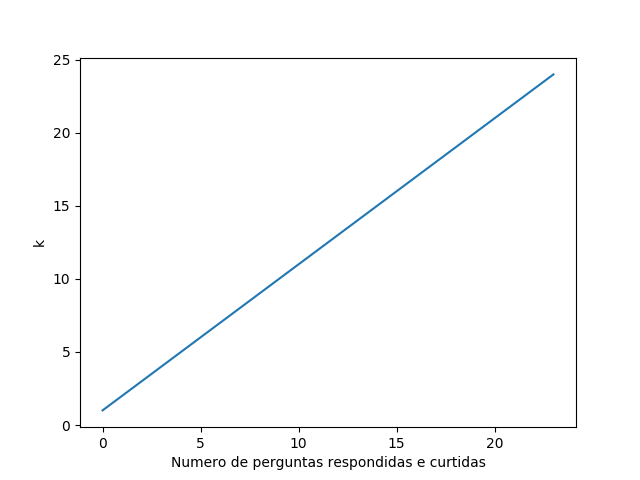
\includegraphics[width=14cm]{grafico_k1.png}
\caption{Evolução de $k$ se todas as perguntas postadas por $A$ forem respondidas por $B$. Fonte: os autores.}
\label{fig:grafico_k1}
\end{figure}

Como o cálculo leva em conta todas as perguntas postadas pelo usuário $A$, no caso de já haver perguntas postadas e não respondidas, o crescimento do valor de $k$ é afetado num grau inversamente proporcional ao número de perguntas postadas, como pode-se observar na Figura \ref{fig:grafico_k2}.

\begin{figure}[!htb]
\centering
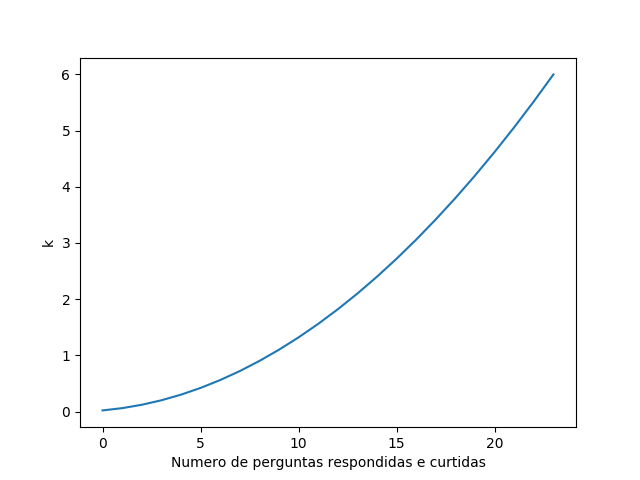
\includegraphics[width=14cm]{grafico_k2.png}
\caption{Evolução de $k$ se $A$ postou 50 perguntas e houve apenas 25 respostas de $B$. Fonte: os autores.}
\label{fig:grafico_k2}
\end{figure}

É importante lembrar que o peso do incremento para $k$ é menor quanto maior for o número de perguntas postadas seja por $A$ ou $B$. Dessa maneira, podemos compreender que a interação entre usuários novos, ou com poucas perguntas postadas, terá influência maior no crescimento do valor de $k$. Por outro lado, a interação entre usuários com muitas perguntas já postadas, incrementará um valor menor sobre $k$.

Tendo calculado um peso para cada aresta que liga os usuários, foi necessário definir um limiar $x$ que seria o valor mínimo de $k$ para considerar que dois usuários são similares o suficiente para serem postos em contato sob o mensageiro instantâneo.

A definição de $x$ provou-se um desafio, tendo em vista que o comportamento de $k$ varia em função do número total de perguntas postadas por dois usuários em análise. A Figura \ref{fig:poucasquestoes} mostra que a convergência para $x = 1$ para o caso de de dois usuários que postaram poucas perguntas é rápida, pois o incremento de $k$ é maior. No caso simulado na Figura \ref{fig:poucasquestoes}, pouco mais de cinco respostas foram o suficiente para atingir o $x$.

\begin{figure}[!htb]
\centering
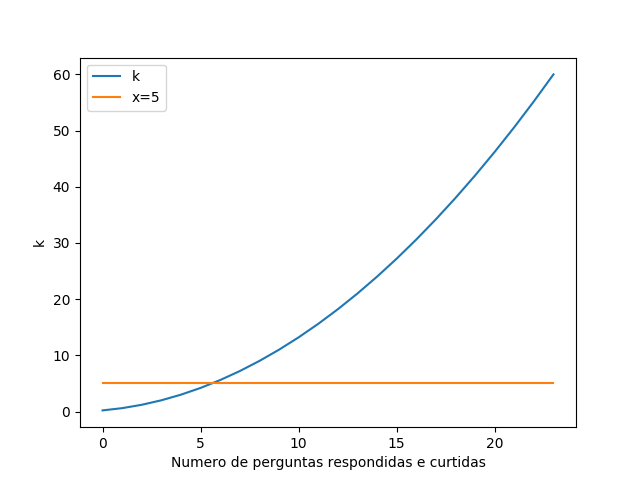
\includegraphics[width=14cm]{poucasquestoes.png}
\caption{Evolução de $k$ em função das respostas curtidas se $A$ e $B$ têm poucas perguntas postadas. Ex.: menos que 10 perguntas. Fonte: os autores.}
\label{fig:poucasquestoes}
\end{figure}

A Figura \ref{fig:muitasquestoes}  demonstra que a convergência de $k$ e $x$ para usuários que já postaram muitas perguntas demanda muito mais respostas, neste caso mais que vinte respostas. Isto deve-se ao fato de ter sido decidido que a equação \ref{eq:k1} tem como divisor a soma de todas as perguntas já postadas pelos dois usuários, portanto, o incremento de $k$ é inversamente proporcional à soma de todas as perguntas postadas pelos usuários. 

\begin{figure}[!htb]
\centering
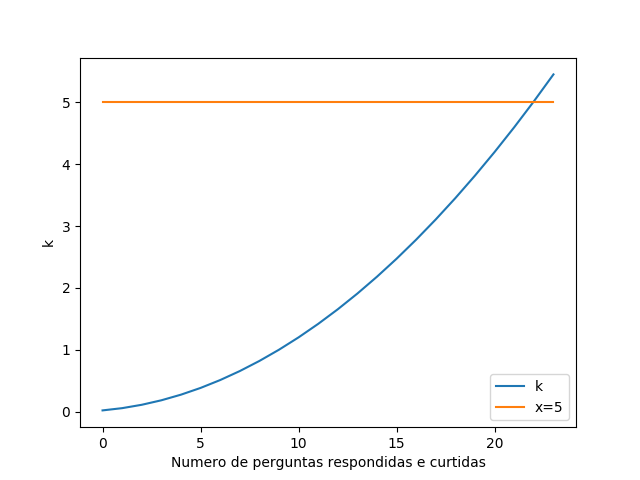
\includegraphics[width=14cm]{muitasquestoes.png}
\caption{Evolução de $k$ em função das respostas se $A$ e $B$ têm muitas perguntas postadas. Ex.: mais que 50 perguntas. Fonte: os autores.}
\label{fig:muitasquestoes}
\end{figure}

Uma adequação simplista para este problema seria definir $k$ como o número total de respostas trocadas entre dois usuários. Assim, $x$ seria o número mínimo de respostas que teriam que ser respondidas entre os usuários para que fossem considerados similares o suficiente para contatarem-se pelo mensageiro instantâneo. Porém, dessa maneira ignora-se que, se houverem muitas perguntas postadas por $A$ sem resposta de $B$ é possível que hajam mais diferenças do que similaridades entre os usuários, haja vista que muitas perguntas são ignoradas.

Portanto, é imprescindível considerar o volume de perguntas postadas e também contabilizar o número de respostas que foram apreciadas pelo usuário que postou a pergunta. Dessa maneira, propomos uma evolução que adequasse o software para contabilizar o número de perguntas postadas por $A$ e \emph{vistas} por $B$, bem como quais respostas cada parte gostou de receber. Assim, poderíamos adequar o cálculo de $k$ como segue: 

\begin{equation}
k = k + \frac{R_{ab} + R_{ba}}{P_{AvB} + P_{BvA}} 
\label{eq:k2}
\end{equation}

Onde $R_{ab}$ é o número de respostas que o usuário $A$ recebeu do usuário $B$ e $A$ gostou; $R_{ba}$ é o número de respostas que o usuário $B$ recebeu do usuário $A$ e a $B$ gostou; $P_{AvB}$ é o número de perguntas postadas pelo usuário $A$ e vistas por $B$ e $P_{BvA}$ o número de respostas postadas pelo usuário $B$ e vistas por $A$.

Aplicando a equação \ref{eq:k2}, o incremento do valor de $k$ para cada resposta curtida seria menor para o caso de muitas perguntas terem sido vistas e poucas respostas terem sido dadas. De maneira inversa, quanto menor o conjunto de perguntas trocadas entre os usuários, maior o peso que uma resposta curtida terá sobre $k$.

Seria conveniente, neste caso, afetar as perguntas postadas com uma validade por cronologia ou fixar um valor máximo para o total de perguntas postadas pelos usuários $A$ e $B$. Para a implementação do produto neste trabalho, não foi considerada a idade das perguntas nem estabelecido um valor limite do somatório de perguntas postadas por $A$ e $B$ pois seria inconveniente para cronograma do desenvolvimento.

Como medida para contornar a dificuldade de implementar um contador para as perguntas que foram vistas por usuários específicos, foi tomada uma aproximação relacionada somente às perguntas respondidas e às respostas apreciadas. A função a seguir define o cálculo de $k$ com essa premissa:

\begin{equation}
k_{ab} = \frac{R_{abA} + R_{baA}}{R_{ab} + R_{ba}} + \frac{R_{ab} + R_{ba}}{P_{a}+P_{b}}
\label{eq:k3}
\end{equation}

Onde $R_{abA}$ e $R_{baA}$ são o número de respostas apreciadas pelo usuário $A$ e $B$, respectivamente; $R_{ab}$ é o número de respostas que $A$ enviou a $B$; $R_{ba}$ é o número de respostas que $B$ enviou a $A$ e, finalmente, $P_{a}$ e $P_{b}$ o número total de perguntas enviadas por $A$ e $B$.

\begin{figure}[!htb]
\centering
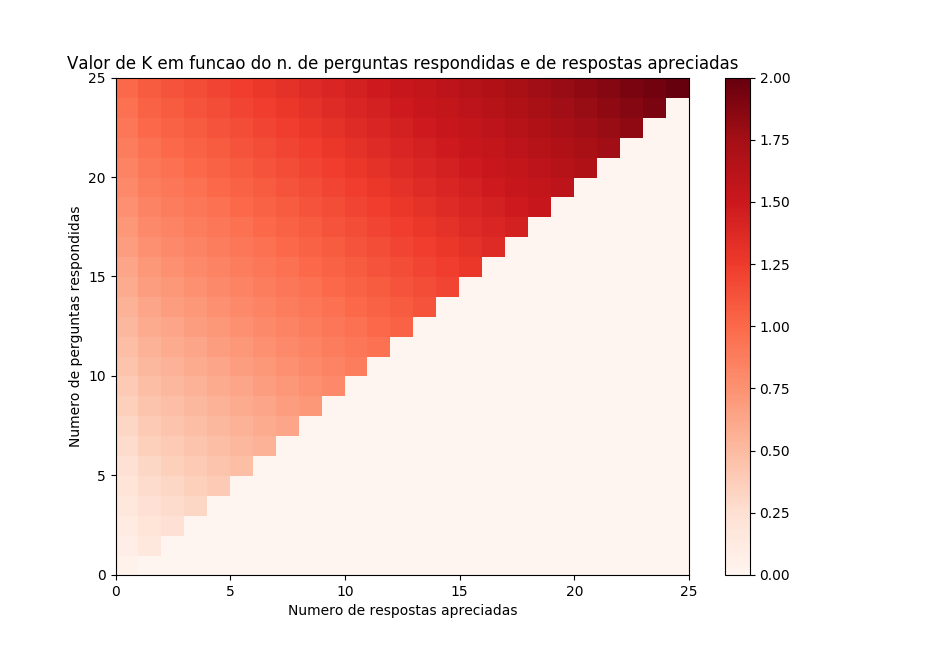
\includegraphics[width=14cm]{matriz_k.png}
\caption{Valor de k em função do número de perguntas respondidas e de respostas curtidas entre dois usuários. Fonte: os autores.}
\label{fig:matrizk}
\end{figure}

Podemos observar na Figura \ref{fig:matrizk} que, aplicando a função \ref{eq:k3}, temos uma correlação entre o número de perguntas respondidas e o número de perguntas apreciadas pelo usuário o que representa uma linearidade desejável no incremento do valor de $k$ proporcionalmente ao número de perguntas que cada usuário respondeu e cada resposta recebida que ele apreciou.

Dessa maneira, o valor de $k$ cresce tanto para perguntas respondidas quanto para respostas apreciadas. Espera-se um incremento maior para cada resposta apreciada pois o divisor deste elemento é o número total de respostas, enquanto para cada resposta sem apreço o divisor é o número total de perguntas.

Dentro deste caso, um valor fixo para $x$, determina um número de respostas e respostas apreciadas entre os usuários proporcional ao número total de perguntas. Nas Figuras \ref{fig:matriz_x} e \ref{fig:matriz_x1}, percebemos que a região que possui $k$ maior que $x=1,5$, por exemplo, tem a mesma área para casos nos quais o número total de perguntas postadas entre dois usuários é 25, que é o caso da Figura \ref{fig:matriz_x}, e 200, que é o caso da Figura \ref{fig:matriz_x1}. Isso implica que o número de perguntas necessárias para atigir $x$ é diretamente proporcional ao número total de perguntas postadas pelos dois usuários.
 
\begin{figure}[!htb]
\centering
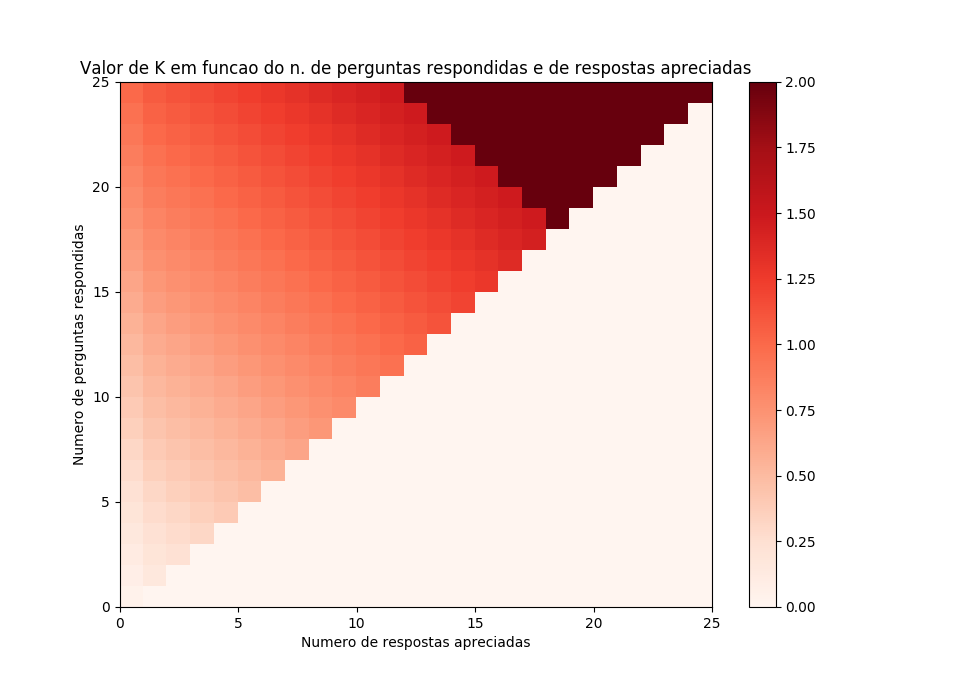
\includegraphics[width=14cm]{matriz_x.png}
\caption{A área em vermelho escuro compreende a relação entre respostas e respostas apreciadas entre dois usuários onde $k$ é maior que 1,5 para 25 perguntas respondidas. Fonte: os autores.}
\label{fig:matriz_x}
\end{figure}

\begin{figure}[!htb]
\centering
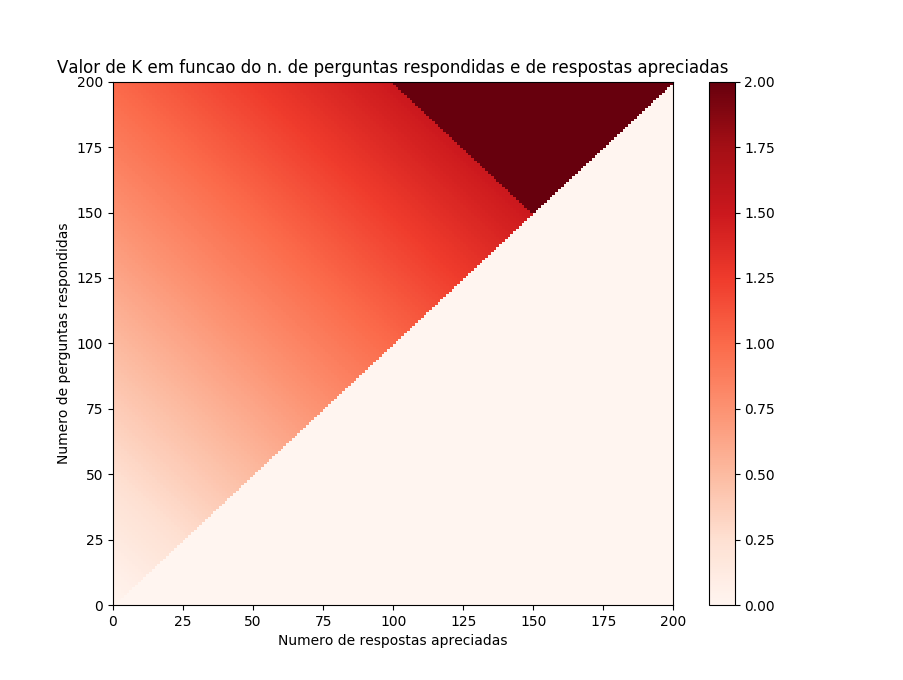
\includegraphics[width=14cm]{matriz_x1.png}
\caption{A área em vermelho escuro compreende a relação entre respostas e respostas apreciadas entre dois usuários onde $k$ é maior que 1,5 para 200 perguntas respondidas. Fonte: os autores.}
\label{fig:matriz_x1}
\end{figure}

A relação entre o número de perguntas postadas e o peso de cada resposta apreciada no cálculo de $k$ é considerada uma funcionalidade interessante para o caso de usuários que já postaram muitas perguntas e encontram similares com facilidade. Consideramos essa ponderação adequada já que facilita a criação de contatos entre usuários recentes e que ainda postaram poucas perguntas e aumenta o desafio para quem já postou muitas perguntas e, possivelmente, já tem muitos contatos desenvolvidos.

Todavia, levando em conta que isto pode desanimar o usuário mais fiel, decidimos não considerar essa ponderação e aplicar uma função que leve em conta apenas o número total de respostas e respostas apreciadas. Aplicamos um fator de multiplicação de cinco para aumentar a influência das respostas que foram apreciadas.

\begin{equation}
k_{ab} = (R_{abA} + R_{baA})*5 + R_{ab} + R_{ba}
\label{eq:k6}
\end{equation}

Porém, considerar as respostas que não foram curtidas pode ser perigoso, uma vez que o usuário que recebe muitas respostas e não aprecia, pode realmente não estar gostando delas e isso culminaria numa proposta de contato desagradável.

Finalmente, foi considerado levar em conta apenas as respostas apreciadas pela razão do número total de respostas. Dessa maneira uma resposta sem apreço é considerada um decremento na força da similaridade calculada pela interação.

\begin{equation}
k_{ab}=(R_{abA}+R_{baA})-\frac{R_{ab}+R_{ba}}{w}
\label{eq:k5}
\end{equation}

Onde $w$ e uma constante que representa o peso dado para o decremento afetado pelo número de perguntas que não foram apreciadas.

Essa função, apesar de simples e elegante, parece ser a mais adequada para a resolução do problema. A equação \ref{eq:k5} considera coerentemente as informações depreendidas do sistema e estabelece uma curva de crescimento apreciável para $k$, independentemente de quantas perguntas já foram postadas, como pode-se observar na Figura \ref{fig:k_ultimaeq}.

\begin{figure}[!htb]
\centering
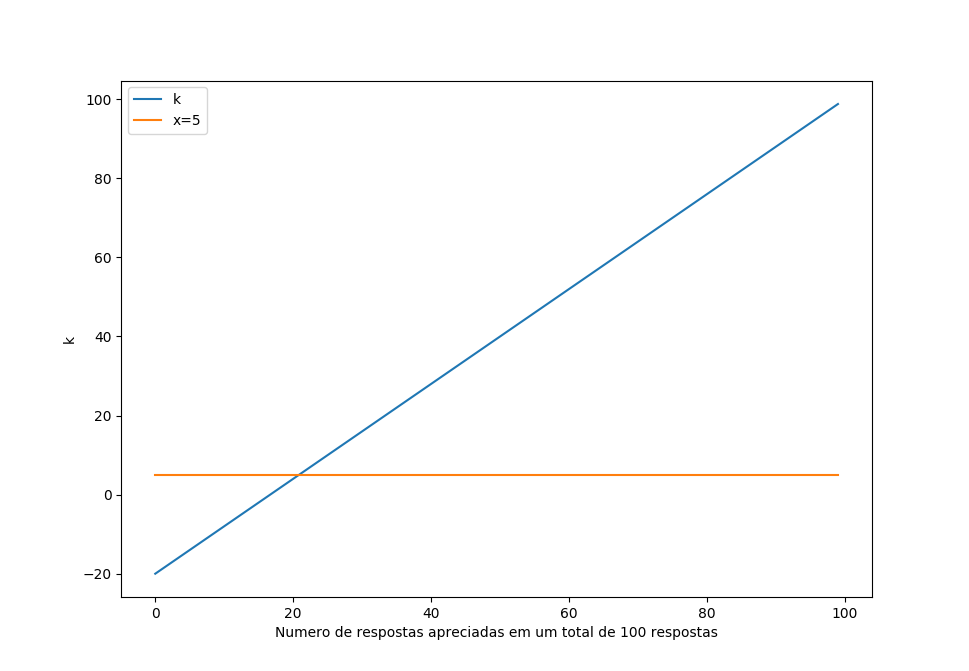
\includegraphics[width=14cm]{k_ultimaeq.png}
\caption{Crescimento de $k$ de acordo com a função \ref{eq:k5} onde $w=5$ e com um limite de $x$ estabelecido em 5. Fonte: os autores.}
\label{fig:k_ultimaeq}
\end{figure}

Os valores de $w$ e $x$ foram estabelecidos considerando um relacionamento mínimo que deve haver para que não seja banalizada a oferta de contatos e para que o usuário mantenha-se interessado no sistema. Esses valores podem ser adaptados por região, datas comemorativas ou campanhas específicas de confraternização que podem ser oferecidas para manter a fidelização.

Outras opções de resolução do problema de sugestão de contatos, poderiam envolver inteligência artificial, algoritmos de classificação ou algoritmos de recomendação.

Um refinamento valioso para a acurácia das recomendações de contatos poderiam envolver o uso de inteligência artificial para fazer uma análise semântica das perguntas e respostas. Dessa maneira, poderíamos depreender um volume muito maior de informações, tanto das perguntas quanto das respostas, a partir de palavras-chave, por exemplo, de maneira que um banco de dados muito mais rico definiria cada usuário. A partir desses dados, um algoritmo de recomendação baseado em filtragem de conteúdo poderia aproximar usuários que costumam escrever sobre assuntos correlatos.

A análise do texto poderia propiciar uma classificação dos usuários a partir de seus interesses e aproximá-los de perguntas que seja mais coerentes com seus gostos. Isso otimizaria a dinâmica de respostas e ofereceria uma experiência mais agradável ao usuário, de maneira que ele sentiria-se familiarizado com as perguntas uma vez que elas seriam selecionadas de acordo com seu interesse.







